\documentclass{standalone}
\usepackage{tikz,bm}
\usetikzlibrary{angles,quotes}
\begin{document}
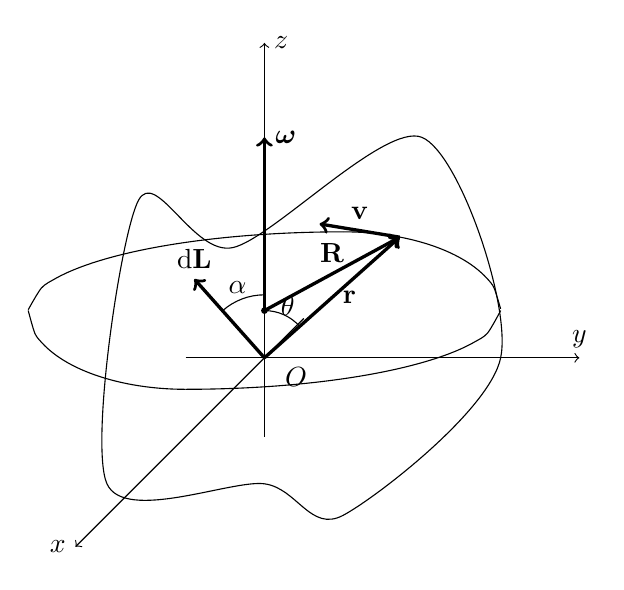
\begin{tikzpicture}[scale=2]
    \coordinate(O)at(0,0);
    \draw[->](-0.5,0)--(2,0)node[above]{$y$};
    \draw[->](0,-0.5)--(0,2)coordinate(z)node[right]{$z$};
    \draw[->](0.25,0.25)--(-1.2,-1.2)node[left]{$x$}; 
    \node[below]at(0.2,0){$O$};

    \draw[->,very thick](0,0)--(0.859,0.766)coordinate(r)node[midway, right]{$\mathbf{r}$};
    \draw[->,very thick](0.859,0.766)--(0.35,0.85)node[midway, above]{$\mathbf{v}$};
    \draw[->,very thick](0,0.3)coordinate(R)--(r)node[midway, above]{$\mathbf{R}$};
    \draw[->,very thick](O)--(-0.445,0.5)coordinate(L)node[above]{$\mathrm{d}\mathbf{L}$};
    \draw[->,very thick](0,0.3)--(0,1.4)node[right]{$\boldsymbol{\omega}$};
    \filldraw[black](0,0.3)circle(0.5pt);

    \draw[-]plot[smooth, domain=-1.5:-0.5](\x,{0.3-0.5*(1-(\x+0.5)^2)^0.5});
    \draw[-]plot[smooth, domain=0.5:1.5](\x,{0.3+0.5*(1-(\x-0.5)^2)^0.5});
    \draw[-]plot[smooth, domain=0.5:-1.5](\x,{0.3+0.25*(4-(\x-0.5)^2)^0.5});
    \draw[-]plot[smooth, domain=1.5:-0.5](\x,{0.3-0.25*(4-(\x+0.5)^2)^0.5});

    \draw[-]plot[smooth cycle]coordinates{(1.5,0)(1,1.4)(-0.2,0.7)(-0.8,1)(-1,-0.8)(0,-0.8)(0.5,-1)};

    \pic["$\alpha$", draw, angle eccentricity=1.2, angle radius=0.8cm]{angle=R--O--L};
    \pic["$\theta$", draw, angle eccentricity=1.2, angle radius=0.6cm]{angle=r--O--R};
\end{tikzpicture}
\end{document}